\documentclass{article}
    % General document formatting
    \usepackage[margin=0.7in]{geometry}
    \usepackage[parfill]{parskip}
    \usepackage[utf8]{inputenc}
    \usepackage{amsmath}
    \usepackage{amssymb}
    \usepackage{tikz}
    \usepackage{fancyhdr}
    \usepackage{listings}

\pagestyle{fancy}
\fancyhf{}
\rhead{Edgar Jacob Rivera Rios - A01184125}

\begin{document}
\begin{titlepage}

    \newcommand{\HRule}{\rule{\linewidth}{0.5mm}} % Defines a new command for the horizontal lines, change thickness here

    \center % Center everything on the page

    %----------------------------------------------------------------------------------------
    %	HEADING SECTIONS
    %----------------------------------------------------------------------------------------

    \textsc{\LARGE Tecnológico de Monterrey}\\[1.5cm] % Name of your university/college
    \textsc{\Large Fundamentos de computación}\\[0.5cm] % Major heading such as course name
    %\textsc{\large Minor Heading}\\[0.5cm] % Minor heading such as course title

    %----------------------------------------------------------------------------------------
    %	TITLE SECTION
    %----------------------------------------------------------------------------------------

    \HRule \\[0.4cm]
    { \huge \bfseries Homework 4}\\[0.4cm] % Title of your document
    \HRule \\[1.5cm]

    %----------------------------------------------------------------------------------------
    %	AUTHOR SECTION
    %----------------------------------------------------------------------------------------

    \begin{minipage}{0.4\textwidth}
    \begin{flushleft} \large
    \emph{Student:}\\
    Jacob \textsc{Rivera} % Your name
    \end{flushleft}
    \end{minipage}
    ~
    \begin{minipage}{0.4\textwidth}
    \begin{flushright} \large
    \emph{Professor:} \\
    Dr. Hugo \textsc{Terashima} % Supervisor's Name
    \end{flushright}
    \end{minipage}\\[2cm]

    % If you don't want a supervisor, uncomment the two lines below and remove the section above
    %\Large \emph{Author:}\\
    %John \textsc{Smith}\\[3cm] % Your name

    %----------------------------------------------------------------------------------------
    %	DATE SECTION
    %----------------------------------------------------------------------------------------

    {\large \today}\\[2cm] % Date, change the \today to a set date if you want to be precise

    %----------------------------------------------------------------------------------------
    %	LOGO SECTION
    %----------------------------------------------------------------------------------------

    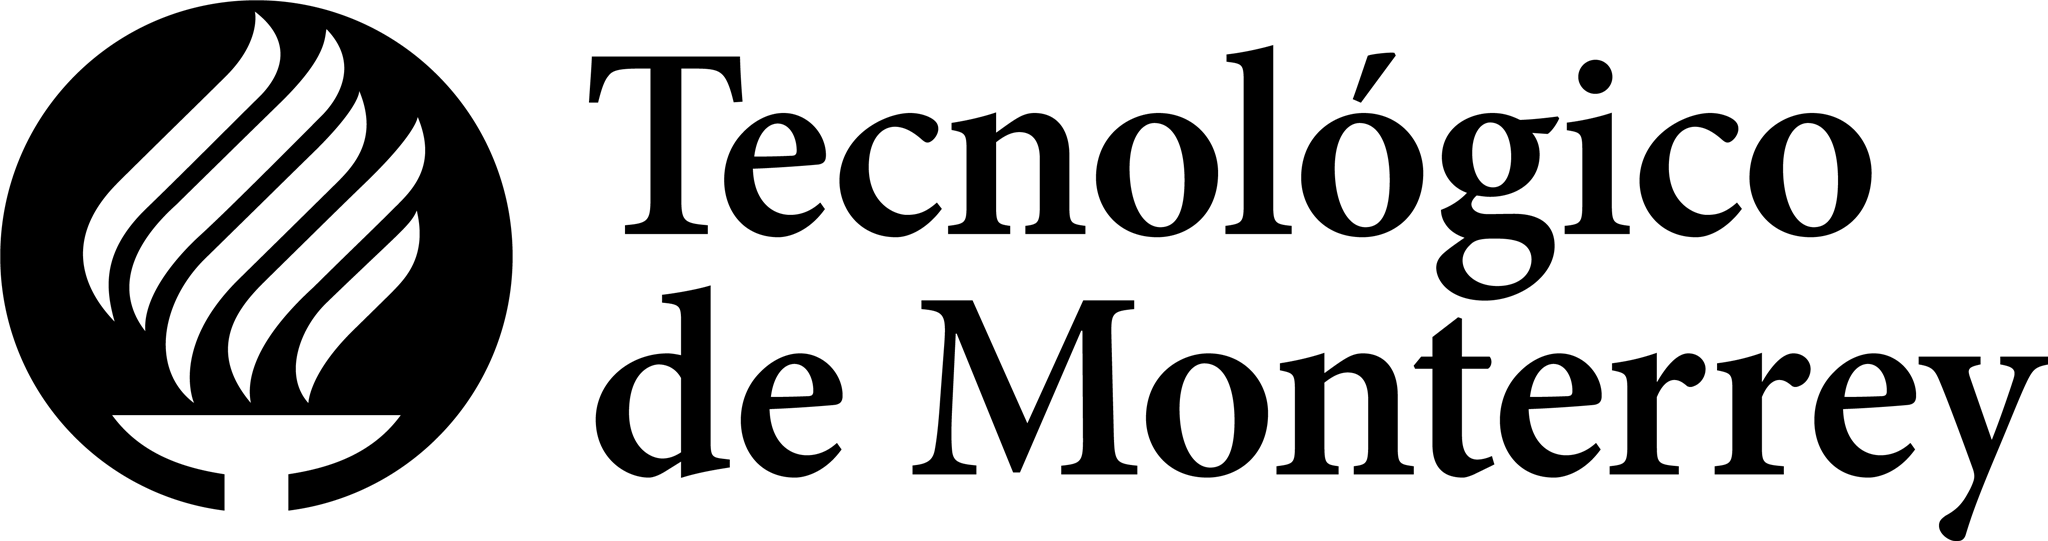
\includegraphics[width=0.4\textwidth,height=\textheight,keepaspectratio]{logo-tec-negro.png} % Include a department/university logo - this will require the graphicx package

    %----------------------------------------------------------------------------------------

    \vfill % Fill the rest of the page with whitespace

\end{titlepage}


\section{Problems}
Solve the following problems:
\begin{enumerate}
    \item Solve problems 4.58 and 4.59 (Sara Baase)

    \item Assume that the subroutine PARTITION within the quicksort algorithm produces a 9-to-1 split. First, generate the recurrence to compute the complexity of the algorithm under these conditions. Second, estimate  the  complexity  of  the  recurrence  and  discuss  if  the unbalance  in  the  partition  makes  the algorithm to loose the optimality.

    \item Show that there is no comparison sorting algorithm whose complexity is linear for at least $n!/2$ inputs of length $n$, What about a fraction $1/n^3$ of inputs of length $n$? What about a fraction $1/2^n$?

    \item Consider an array of characters $R$, $W$, y $B$, and you want to arrange the array in such a way that the $R$s are first, then the $W$s, and at the end the $B$s. Describe a linear algorithm to accomplish this task.

    \item Take a sequence of $2n$ numbers as input. Design an algorithm that partitions the numbers into $n$ pairs, with the property that the partition minimizes the maximum sum of the pair. For example, say we are given the numbers (1,3,5,9). The possible partitions are ((1,3),(5,9)), ((1,5), (3,9)) and((1,9),(3,5)). The pair sums of these partitions are (4,14), (6,12) y (10,8). Thus the third partition has 10 as its maximum sum, which is the minimum over the three partitions. Establish the complexity of your algorithm.
\end{enumerate}
\end{document}